\documentclass[12pt, letterpaper]{article}

\usepackage{amsmath} % needed for including equations
\usepackage[margin=1in]{geometry} % sets the margins to 1in
\usepackage{graphicx} % needed for figures
\graphicspath{{./figures/}} % allows figures to be placed in a different folder
\usepackage[hang,small,bf]{caption} % sets the style on the figure captions
\usepackage{epstopdf} % converts eps files to pdf to display in the latex document



\begin{document}

\begin{titlepage}

\begin{center}

\vspace*{\fill}

\vspace{0.5in}

% Insert your title here
{ \LARGE \bfseries Title of Your Prospectus}\\[.25in]

\large
by\\[.25 in]
% Change your name here
Your Name\\[1in]

A prospectus submitted to the faculty of\\
Department of Mechanical Engineering\\
Brigham Young University

\vspace{1in}

\today

\vspace*{\fill}

\end{center}

\end{titlepage}

\thispagestyle{empty}

\begin{center}
\vspace*{\fill}

\begin{figure}[htbp] %  figure placement: here, top, bottom, or page
   \centering
   
\includegraphics[width=2.5in]{byume_logo_clear.jpg} 
\end{figure}

\vspace{0.5in}

\Large{Prospectus Approval}\\[0.5in]

\end{center}

\hspace*{.47in}
\begin{minipage}[c]{5.25in}

\normalsize

Prospectus submitted by:

\vspace{.5in}

\makebox[2in]{\hrulefill} \hspace{1in} \makebox[2in]{\hrulefill}

% Change your name here
\parbox[b]{3in}{Your name} \, Date
\vspace{0.5in}

This prospectus has been approved by each member of the Graduate Committee:
\vspace{0.5in}

\makebox[2in]{\hrulefill} \hspace{1in} \makebox[2in]{\hrulefill}

\parbox[b]{3in}{Committee Member - Chair} \, Date
\vspace{0.4in}

\makebox[2in]{\hrulefill} \hspace{1in} \makebox[2in]{\hrulefill}

\parbox[b]{3in}{Committee Member} \, Date
\vspace{0.4in}

\makebox[2in]{\hrulefill} \hspace{1in} \makebox[2in]{\hrulefill}

\parbox[b]{3in}{Committee Member} \, Date

\end{minipage}

\vspace*{\fill}

\pagebreak

\setcounter{page}{1}

\section{Problem Statement}

Gas turbine engines (GTEs) are prevalent in aircraft propulsion and power generation. Efforts are continuously being made to increase their efficiency. One proposed means to increase the efficiency of the conventional GTE is to use a pulse detonation engine (PDE) in place of the combustor. The past 10 years have shown an increased interest in PDEs, especially since the Air Force Research Laboratory at Wright-Patterson Air Force Base demonstrated the viability of using a PDE to propel an aircraft in 2008 \cite{Barr2008}. The integration of PDEs into GTEs shows potential for improvement in both efficiency \cite{Rasheed2011:Experimental} and simplicity \cite{Povinelli2002:PulseDetonation, Hutchins2003:EnergyandExergy}. The pulse detonation cycle consists of pressure-gain combustion and would eliminate the need for as many compressor stages since the additional pressure rise can be achieved in the combustion chamber \cite{Glaser2007:Performance, Hofer2009:Performance}. However, pulse detonations result in high pressure pulses and unsteady flow into the turbine. These phenomena are not currently understood very well.

For PDEs to be successfully used to drive a turbine, it is necessary to better understand turbine performance under unsteady, pulsed conditions.

%The compressor in gas turbine engines runs with an adverse pressure gradient. If the needed pressure gain could be obtained in a different manner, improvements in overall efficiency could be realized. Pressure-gain combustion in the form of pulse detonations provides this solution. \cite{hofer:2009performance-met}

%Glaser et. al. 2007 \cite{glaser:2007performance-of-}
%Combining a PDE with a GTE has the potential to increase the efficiency of the engine. Detonation combustion is pressure-gain combustion that approximates a constant-volume process. The pressure-gain combustion characteristic also eliminates the need for as many compressor stages since the PDE only requires enough air pressure to fill and purge the tubes and does not require as high a pressure as a conventional GTE.

\section{Background}

%Rouser 2011 Performance \cite{Rouser2011:Performance}
Detonation is a pressure-gain, near constant-volume combustion process. The pulse detonation cycle consists of three main events: fill, fire, and purge \cite{Rouser2011:Performance}. Figure~\ref{fig:PDEcycle} visually shows the pulse detonation cycle described below.

\begin{enumerate}
\item During the fill stage a fuel-air mixture enters the pulse detonation tube.
\item The fire stage is further divided into four events. First, the fuel-air mixture is ignited. Second, the deflagration transitions to a detonation. This is known as deflagration to detonation transition (DDT) and can be hastened by physical barriers such as spirals. Third, the detonation propagates down the length of the tube. Fourth, rarefaction waves exhaust the combustion products from the tube in a process known as blow down.
\item During the final stage of the pulse detonation cycle, or the purge stage, air enters the tube to push the rest of the exhaust products from the tube and to provide air for the next combustion event.
\end{enumerate}

\begin{figure}[htbp] %  figure placement: here, top, bottom, or page
   \centering
   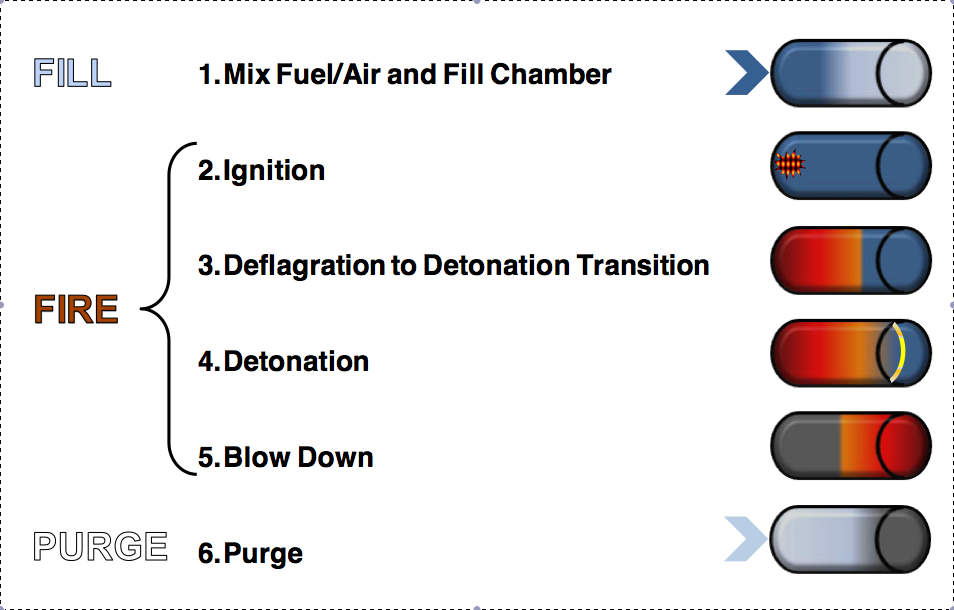
\includegraphics[trim = 5mm 5mm 5mm 5mm,clip,width=4in]{PDEcycle.png} 
   \caption{The PDE cycle as presented by Rouser et. al. \cite{Rouser2011:Performance}.}
   \label{fig:PDEcycle}
\end{figure}

%Hutchins and Metghalchi 2003
Hutchins and Metghalchi \cite{Hutchins2003:EnergyandExergy} used the Humphrey cycle, which is a constant-volume cycle, to numerically approximate the PDE cycle. The results were compared with a Brayton cycle. The Humphrey cycle shows an increase in efficiency over the Brayton cycle between 4 and 12\%. Since both cycles were modeled in a similar manner, this study provides a good comparison, although it should not be taken as representative of the real cycles.

%Rahseed et. al. 2005
In 2005, Rasheed et. al. \cite{Rasheed2005:Experimental} performed a study using a 14" diameter single stage axial turbine driven by 8 pulsed detonation tubes arranged in a can-annular configuration. The pulse detonation tubes were operated at frequencies of 10, 20, and 30 Hz and were fired in two different configurations, sequentially and simultaneously. However, there was no comparison made to steady flow.

%Rahseed et. al. 2011
Six years later Rasheed et. al. \cite{Rasheed2011:Experimental} conducted another study using a similar setup to the study mentioned above. Four different types of tests were performed. First, the turbine was installed in its native configuration and driven by the steady flow of air at atmospheric conditions. Second, the turbine was placed in the experimental rig and driven by heated air. Third, a steady burner was placed upstream of the turbine to simulate the steady deflagration flow in an actual GTE. Fourth, pulse detonations were fired into the turbine. For the pulse detonation firing condition both sequential and simultaneous firing was performed. The turbine work was measured using the compressor work and correcting for frictional losses in the bearings. No distinction in turbine performance could be determined within the uncertainty of the instrumentation. This might be due to the bypass air used to cool the pulse detonation tubes. The pulse detonation tubes shared a common air inlet as well as an exit. This common exit is 4.2 inches long and allows for some mixing before the air enters the turbine. However, when the efficiency of the entire rig was estimated, the pulse detonation driven turbine showed a four point increase in overall efficiency from steady state operation.

%Glaser et. al. 2007 \cite{Glaser2007:Performance}
Glaser et. al. \cite{Glaser2007:Performance} also compared results of a turbine driven by pulse detonation and constant-pressure deflagration. Both of these combustion methods were performed in the same tubes which exhausted into the turbine. The data showed that the efficiency of the pulse detonation driven turbine was comparable to the efficiency of the steady burner driven turbine. It is important to note there was a gap of approximately 7 tube diameters between the pulse detonation tube exit and the turbine inlet where mixing with bypass air occurred, which would allow for shock dissipation. Only a maximum of 21\% of the total turbine mass flow was combustion gases.

\section{Research Objectives}

Previous experimental studies with a turbine driven by pulsed detonations all had a bypass region where the detonation exhaust mixed with ambient air before passing through the turbine. The bypass air was used to cool the combustion products before entering the turbine. Cooling of the air is necessary for the small turbines used in research because these small turbines do not have cooling mechanisms such as those employed in larger GTEs. However, mixing the pulses with bypass air will dampen the effect of the pulses on turbine performance. The proposed research will use compressed air instead of combustion products to produce both steady and pulsed flow. Not employing combustion in the proposed research will eliminate the need for bypass cooling air. Without the need for cooling air, which would dampen the pressure pulses entering the turbine, a more direct comparison of turbine performance under steady and pulsed flow will be made.

The proposed work will accomplish the following objectives:

\begin{itemize}

	\item Design and build an experimental test rig to provide steady (simulate traditional turbine operation) and unsteady (simulate PDE driven turbine) flow to an axial turbine.

	\item Determine a compressed air profile that best represents normal steady flow and pulsed detonation flow conditions.

	\item Experimentally measure turbine performance under steady and pulsed flow.

	\item Compare the collected data by creating a turbine map for both steady and pulsed flow. Specific power will also be used to compare turbine performance under steady and pulsed flow.

\end{itemize}

\section{Proposed Research}

An experimental test rig capable of providing both steady and unsteady flow through the axial turbine of a JetCat P-200 gas turbine engine will be designed and built. The JetCat P-200 engine is a hobbyist jet engine with a single stage radial compressor and a single stage axial turbine. The engine runs at speeds between 32000 and 112000 rpm, has a maximum thrust of 52 lbs, a mass flow rate of 1 lbm/min, and weighs 5 lbs \cite{jetcat}. In lieu of a combustor, the engine will be modified to allow compressed air to be ducted into the turbine.

A compressed air pressure profile that best approximates pulse detonation flow through the turbine was determined. Figure~\ref{fig:pressurecomparison} compares the turbine inlet pressure from a PDE operated with cold flow (no combustion) with flow through a ball valve rotated with an electric motor. The goal in simulating PDE flow is to produce periodic pressure pulses which are qualitatively similar to actual PDE flow. While the patterns are not identical, the flow through the rotating ball valve is a good qualitative approximation of PDE flow without combustion as can be seen in Figure~\ref{fig:pressurecomparison}. Fired PDE operation would have pressure pulses with a much greater amplitude due to detonations. This greater amplitude can be simulated with a rotating ball valve by increasing the pressure of the air upstream of the ball valve. The pressure spike from the detonation wave in a PDE operated at 15 Hz has an amplitude of 9.2 atm \cite{Rouser2011:Time-Accurate}. At 12.3 Hz, the simulated flow has an amplitude of 6 atm. Again, the simulated flow does not exactly match the actual fired PDE flow, but does provide a qualitative approximation. 

\begin{figure}[htbp] %  figure placement: here, top, bottom, or page
   \centering
   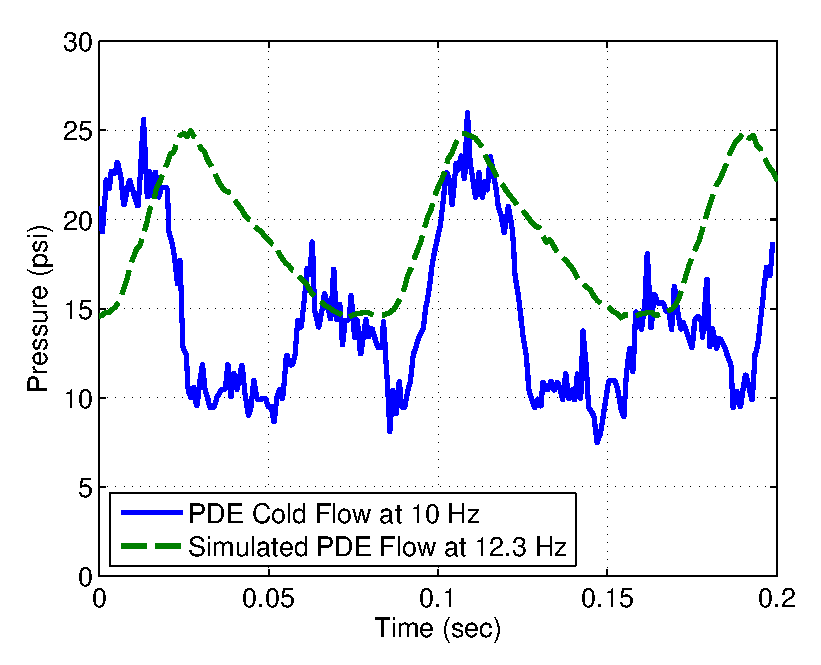
\includegraphics[trim = 0mm 0mm 0mm 0mm,clip,width=4in]{pressure.eps}
   \caption{Comparison of actual and simulated PDE flow. The solid blue line is the turbine inlet pressure for cold flow as presented by Rouser et. al. \cite{Rouser2010:Unsteady}. The dashed green line is the exit pressure from a valve rotated at 12.3~Hz. The peaks are not aligned due to the different operating frequencies. This figure shows that a rotating ball valve can be used to qualitatively approximate PDE flow through a turbine.}
   \label{fig:pressurecomparison}
\end{figure}

The experimental apparatus will have instrumentation to measure pressures, temperatures, and mass flow.
%The pressures and temperatures will be measured at the turbine and compressor inlets and outlets. Pressures will be measured using pressure transducers and temperatures using thermocouples. The thrust will be measured using an air bearing system to decrease friction and a strain gauge. The mass flow into the compressor and turbine will be measured.
Turbine power will be measured using the compressor work. Exact power measurement is not necessary since a comparison will be made on the same equipment and not with independently collected data.

Experimental data will be used to compare steady and pulsed flow. Comparisons will be made using specific power, turbine efficiency, and a turbine map. Specific thrust and power will both be calculated by dividing the respective quantities by the mass flow rate through the turbine. The conventional methods used to calculate turbine efficiency are not adequate due to the unsteady flow conditions. A method to include the unsteady effects in the calculation of efficiency is still being investigated.

An example of an equation is shown in Equation~\ref{eq:efficiency}.

\begin{equation}
\eta_t = \cfrac{\dot W_c + \dot W_{fric}}{\dot m c_p \left[ 1 - \left( \cfrac{p_{t5}}{p_{t4}} \right)^\frac{\gamma - 1}{\gamma} \right]}
\label{eq:efficiency}
\end{equation}

%Flack \cite{flack:2008fundamentals-of} presents a method to create a turbine map. Both turbine pressure ratio and efficiency can be expressed as functions of corrected mass flow and rotational speed as shown in Equations~\ref{pressure_ratio} and~\ref{efficiency_function}.
%
%\begin{equation}
%\frac{p_{t4}}{p_{t5}} = \mathscr{F} \left\{ \frac{\dot m \sqrt{\theta_{t4}}}{\delta_{t4}}, \frac{N}{\sqrt{\theta_{t4}}} \right\} = \mathscr{F} \left\{ \dot m_{c4}, N_{c4} \right\}
%\label{pressure_ratio}
%\end{equation}
%%
%\begin{equation}
%\eta = \mathscr{G} \left\{ \frac{\dot m \sqrt{\theta_{t4}}}{\delta_{t4}} , \frac{N}{\sqrt{\theta_{t4}}} \right\} = \mathscr{G} \left\{ \dot m_{c4}, N_{c4} \right\}
%\label{efficiency_function}
%\end{equation}
%%
%where
%\[\delta_{t4} = p_{t4}/p_{stp}\]
%and
%\[\theta_{t4} = T_{t4}/T_{stp}\]
%%
%Lines of constant corrected speed and efficiency will then be plotted on an axis of pressure ratio versus corrected mass flow.

\section{Anticipated Contributions}

As a result of this research, there will be an improved understanding of the effect of unsteady, pulsed flow through a turbine. A direct comparison will be made between steady and unsteady flow through an axial turbine without any bypass flow. This direct comparison has not been previously performed. Possible publications from this research include presenting at the ASME Turbo Expo, submitting to the ASME Journal of Turbomachinery, presenting at the AIAA Aerospace Science Meeting, or other conferences and journals. This research is sponsored by Innovative Scientific Solutions, Inc. through an Air Force contract.


\pagebreak

\bibliographystyle{IEEEtran}
\bibliography{library}

\end{document}